\documentclass{standalone}
\usepackage{tikz}
\usetikzlibrary{patterns, positioning}
\usepackage[sfdefault]{ClearSans} %% option 'sfdefault' activates Clear Sans as the default text font
\usepackage[T1]{fontenc}

\begin{document}
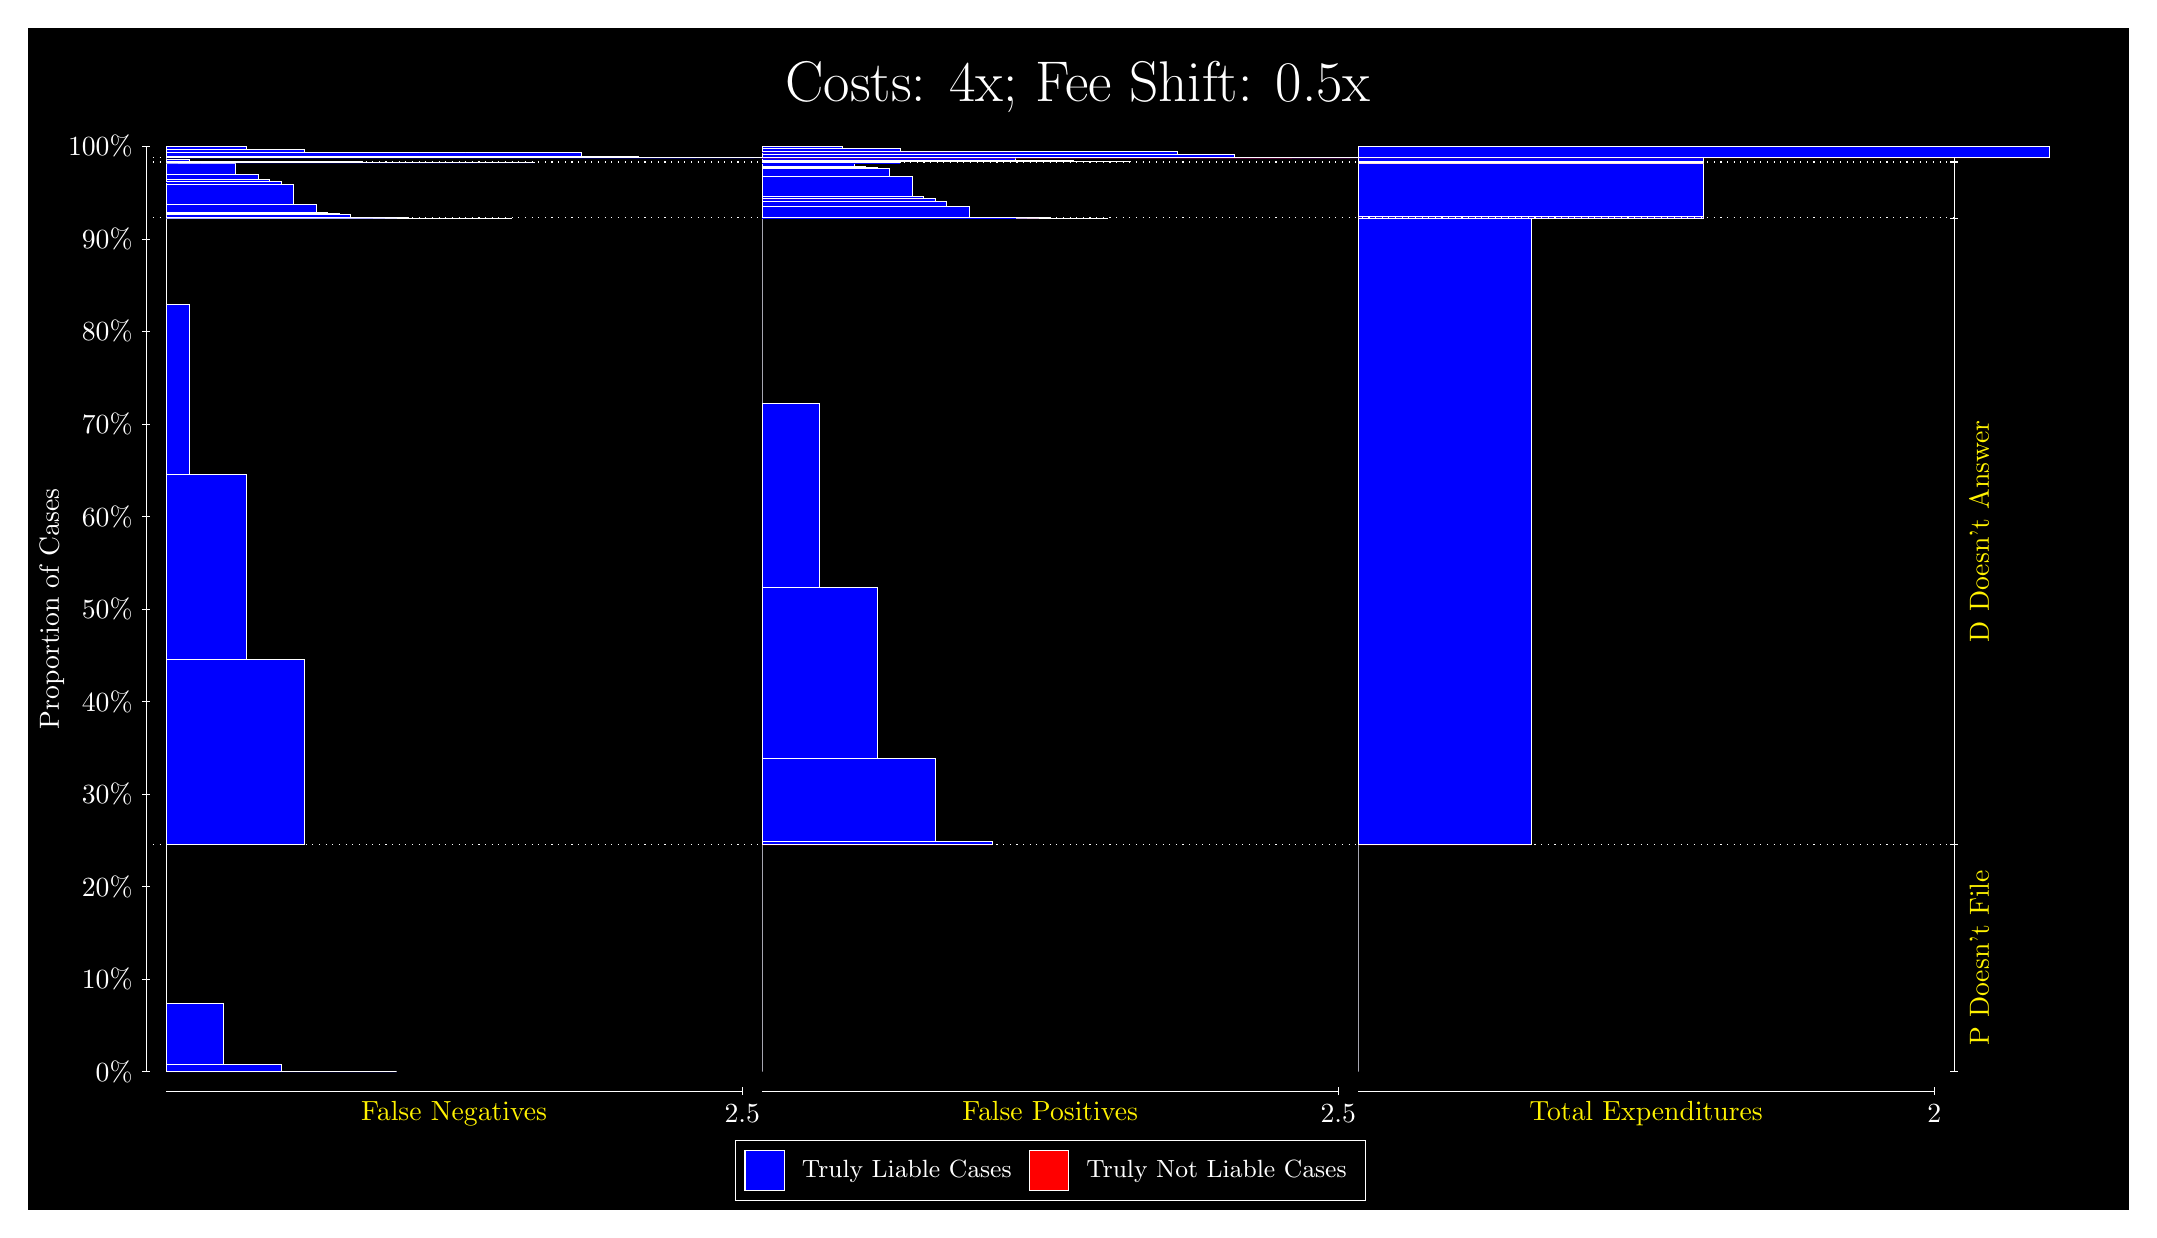
\begin{tikzpicture}
\draw[fill=black] (0,0) rectangle (26.667,15);
\draw[text=white] (0,13.5) rectangle (26.667,15) node[midway] {\huge Costs: 4x; Fee Shift: 0.5x};
\draw[white, very thin] (1.5,1.75) -- (1.5,13.5);
\node[rotate=90, text=white, anchor=center] at (0.3, 7.625) {Proportion of Cases};
\draw[white, very thin] (1.45,1.75) -- (1.55,1.75);
\node[text=white, anchor=east] at (1.45, 1.75) {0\%};
\draw[white, very thin] (1.45,2.925) -- (1.55,2.925);
\node[text=white, anchor=east] at (1.45, 2.925) {10\%};
\draw[white, very thin] (1.45,4.1) -- (1.55,4.1);
\node[text=white, anchor=east] at (1.45, 4.1) {20\%};
\draw[white, very thin] (1.45,5.275) -- (1.55,5.275);
\node[text=white, anchor=east] at (1.45, 5.275) {30\%};
\draw[white, very thin] (1.45,6.45) -- (1.55,6.45);
\node[text=white, anchor=east] at (1.45, 6.45) {40\%};
\draw[white, very thin] (1.45,7.625) -- (1.55,7.625);
\node[text=white, anchor=east] at (1.45, 7.625) {50\%};
\draw[white, very thin] (1.45,8.8) -- (1.55,8.8);
\node[text=white, anchor=east] at (1.45, 8.8) {60\%};
\draw[white, very thin] (1.45,9.975) -- (1.55,9.975);
\node[text=white, anchor=east] at (1.45, 9.975) {70\%};
\draw[white, very thin] (1.45,11.15) -- (1.55,11.15);
\node[text=white, anchor=east] at (1.45, 11.15) {80\%};
\draw[white, very thin] (1.45,12.325) -- (1.55,12.325);
\node[text=white, anchor=east] at (1.45, 12.325) {90\%};
\draw[white, very thin] (1.45,13.5) -- (1.55,13.5);
\node[text=white, anchor=east] at (1.45, 13.5) {100\%};

\draw[white, very thin] (24.457,1.75) -- (24.457,13.5);
\draw[white, very thin] (24.407,1.75) -- (24.507,1.75);
\node[anchor=west] at (24.407, 1.75) {};
\draw[white, very thin] (24.407,4.6314) -- (24.507,4.6314);
\node[anchor=west] at (24.407, 4.6314) {};
\draw[white, very thin] (24.407,12.592) -- (24.507,12.592);
\node[anchor=west] at (24.407, 12.592) {};
\draw[white, very thin] (24.407,13.292) -- (24.507,13.292);
\node[anchor=west] at (24.407, 13.292) {};
\draw[white, very thin] (24.407,13.309) -- (24.507,13.309);
\node[anchor=west] at (24.407, 13.309) {};
\draw[white, very thin] (24.407,13.356) -- (24.507,13.356);
\node[anchor=west] at (24.407, 13.356) {};
\draw[white, very thin] (24.407,13.5) -- (24.507,13.5);
\node[anchor=west] at (24.407, 13.5) {};

\draw[white, very thin, fill=blue] (1.75,1.75) rectangle (4.6775,1.75);
\draw[white, very thin, fill=blue] (1.75,1.75) rectangle (3.9457,1.7508);
\draw[white, very thin, fill=blue] (1.75,1.7508) rectangle (3.2138,1.8459);
\draw[white, very thin, fill=blue] (1.75,1.8459) rectangle (2.4819,2.6153);
\draw[white, very thin, fill=red] (1.75,2.6153) rectangle (1.75,2.6153);
\draw[white, very thin, fill=blue] (1.75,2.6153) rectangle (1.75,4.6314);
\draw[white, very thin, fill=blue] (1.75,4.6314) rectangle (3.5065,6.9813);
\draw[white, very thin, fill=blue] (1.75,6.9813) rectangle (2.7746,9.3297);
\draw[white, very thin, fill=blue] (1.75,9.3297) rectangle (2.0428,11.491);
\draw[white, very thin, fill=red] (1.75,11.491) rectangle (1.75,11.491);
\draw[white, very thin, fill=blue] (1.75,11.491) rectangle (1.75,12.592);
\draw[white, very thin, fill=blue] (1.75,12.592) rectangle (6.1413,12.592);
\draw[white, very thin, fill=blue] (1.75,12.592) rectangle (5.8486,12.592);
\draw[white, very thin, fill=blue] (1.75,12.592) rectangle (5.5558,12.592);
\draw[white, very thin, fill=blue] (1.75,12.592) rectangle (5.4094,12.592);
\draw[white, very thin, fill=blue] (1.75,12.592) rectangle (5.2631,12.592);
\draw[white, very thin, fill=blue] (1.75,12.592) rectangle (5.1167,12.592);
\draw[white, very thin, fill=blue] (1.75,12.592) rectangle (4.9703,12.592);
\draw[white, very thin, fill=blue] (1.75,12.592) rectangle (4.8239,12.593);
\draw[white, very thin, fill=blue] (1.75,12.593) rectangle (4.6775,12.593);
\draw[white, very thin, fill=blue] (1.75,12.593) rectangle (4.5312,12.593);
\draw[white, very thin, fill=blue] (1.75,12.593) rectangle (4.3848,12.593);
\draw[white, very thin, fill=blue] (1.75,12.593) rectangle (4.3848,12.598);
\draw[white, very thin, fill=blue] (1.75,12.598) rectangle (4.2384,12.598);
\draw[white, very thin, fill=blue] (1.75,12.598) rectangle (4.092,12.633);
\draw[white, very thin, fill=blue] (1.75,12.633) rectangle (4.092,12.633);
\draw[white, very thin, fill=blue] (1.75,12.633) rectangle (3.9457,12.656);
\draw[white, very thin, fill=blue] (1.75,12.656) rectangle (3.7993,12.663);
\draw[white, very thin, fill=blue] (1.75,12.663) rectangle (3.6529,12.663);
\draw[white, very thin, fill=blue] (1.75,12.663) rectangle (3.6529,12.761);
\draw[white, very thin, fill=blue] (1.75,12.761) rectangle (3.5065,12.765);
\draw[white, very thin, fill=blue] (1.75,12.765) rectangle (3.3602,13.02);
\draw[white, very thin, fill=blue] (1.75,13.02) rectangle (3.3602,13.02);
\draw[white, very thin, fill=blue] (1.75,13.02) rectangle (3.2138,13.051);
\draw[white, very thin, fill=blue] (1.75,13.051) rectangle (3.0674,13.053);
\draw[white, very thin, fill=blue] (1.75,13.053) rectangle (3.0674,13.079);
\draw[white, very thin, fill=blue] (1.75,13.079) rectangle (2.921,13.08);
\draw[white, very thin, fill=blue] (1.75,13.08) rectangle (2.921,13.143);
\draw[white, very thin, fill=blue] (1.75,13.143) rectangle (2.7746,13.151);
\draw[white, very thin, fill=blue] (1.75,13.151) rectangle (2.6283,13.283);
\draw[white, very thin, fill=blue] (1.75,13.283) rectangle (2.6283,13.283);
\draw[white, very thin, fill=blue] (1.75,13.283) rectangle (2.4819,13.289);
\draw[white, very thin, fill=blue] (1.75,13.289) rectangle (2.3355,13.289);
\draw[white, very thin, fill=blue] (1.75,13.289) rectangle (2.3355,13.291);
\draw[white, very thin, fill=blue] (1.75,13.291) rectangle (2.1891,13.291);
\draw[white, very thin, fill=blue] (1.75,13.291) rectangle (2.0428,13.292);
\draw[white, very thin, fill=blue] (1.75,13.292) rectangle (1.8964,13.292);
\draw[white, very thin, fill=red] (1.75,13.292) rectangle (1.75,13.292);
\draw[white, very thin, fill=blue] (1.75,13.292) rectangle (1.75,13.292);
\draw[white, very thin, fill=blue] (1.75,13.292) rectangle (6.4341,13.292);
\draw[white, very thin, fill=blue] (1.75,13.292) rectangle (5.7022,13.292);
\draw[white, very thin, fill=blue] (1.75,13.292) rectangle (4.9703,13.296);
\draw[white, very thin, fill=blue] (1.75,13.296) rectangle (4.2384,13.308);
\draw[white, very thin, fill=blue] (1.75,13.308) rectangle (3.5065,13.309);
\draw[white, very thin, fill=red] (1.75,13.309) rectangle (1.75,13.309);
\draw[white, very thin, fill=blue] (1.75,13.309) rectangle (3.5065,13.309);
\draw[white, very thin, fill=blue] (1.75,13.309) rectangle (2.7746,13.309);
\draw[white, very thin, fill=blue] (1.75,13.309) rectangle (2.0428,13.338);
\draw[white, very thin, fill=red] (1.75,13.338) rectangle (1.75,13.338);
\draw[white, very thin, fill=blue] (1.75,13.338) rectangle (1.75,13.356);
\draw[white, very thin, fill=blue] (1.75,13.356) rectangle (9.9471,13.356);
\draw[white, very thin, fill=blue] (1.75,13.356) rectangle (9.2152,13.356);
\draw[white, very thin, fill=blue] (1.75,13.356) rectangle (8.4834,13.356);
\draw[white, very thin, fill=blue] (1.75,13.356) rectangle (7.7515,13.375);
\draw[white, very thin, fill=blue] (1.75,13.375) rectangle (7.0196,13.423);
\draw[white, very thin, fill=blue] (1.75,13.423) rectangle (6.2877,13.423);
\draw[white, very thin, fill=blue] (1.75,13.423) rectangle (5.7022,13.423);
\draw[white, very thin, fill=blue] (1.75,13.423) rectangle (5.5558,13.423);
\draw[white, very thin, fill=blue] (1.75,13.423) rectangle (4.9703,13.423);
\draw[white, very thin, fill=blue] (1.75,13.423) rectangle (4.2384,13.424);
\draw[white, very thin, fill=blue] (1.75,13.424) rectangle (3.5065,13.458);
\draw[white, very thin, fill=blue] (1.75,13.458) rectangle (2.7746,13.496);
\draw[white, very thin, fill=blue] (1.75,13.496) rectangle (2.0428,13.5);
\draw[white, very thin, fill=red] (1.75,13.5) rectangle (1.75,13.5);
\draw[white, very thin, fill=blue] (1.75,13.5) rectangle (1.75,13.5);
\draw[white, very thin, fill=red] (9.3189,1.75) rectangle (9.3189,1.75);
\draw[white, very thin, fill=blue] (9.3189,1.75) rectangle (9.3189,4.6314);
\draw[white, very thin, fill=red] (9.3189,4.6314) rectangle (12.246,4.6314);
\draw[white, very thin, fill=blue] (9.3189,4.6314) rectangle (12.246,4.6784);
\draw[white, very thin, fill=blue] (9.3189,4.6784) rectangle (11.515,5.7331);
\draw[white, very thin, fill=blue] (9.3189,5.7331) rectangle (10.783,7.8941);
\draw[white, very thin, fill=blue] (9.3189,7.8941) rectangle (10.051,10.243);
\draw[white, very thin, fill=blue] (9.3189,10.243) rectangle (9.3189,12.592);
\draw[white, very thin, fill=red] (9.3189,12.592) rectangle (13.71,12.592);
\draw[white, very thin, fill=blue] (9.3189,12.592) rectangle (13.71,12.592);
\draw[white, very thin, fill=red] (9.3189,12.592) rectangle (13.417,12.592);
\draw[white, very thin, fill=blue] (9.3189,12.592) rectangle (13.417,12.592);
\draw[white, very thin, fill=red] (9.3189,12.592) rectangle (13.125,12.592);
\draw[white, very thin, fill=blue] (9.3189,12.592) rectangle (13.125,12.592);
\draw[white, very thin, fill=blue] (9.3189,12.592) rectangle (12.978,12.593);
\draw[white, very thin, fill=red] (9.3189,12.593) rectangle (12.832,12.593);
\draw[white, very thin, fill=blue] (9.3189,12.593) rectangle (12.832,12.593);
\draw[white, very thin, fill=blue] (9.3189,12.593) rectangle (12.686,12.593);
\draw[white, very thin, fill=red] (9.3189,12.593) rectangle (12.539,12.593);
\draw[white, very thin, fill=blue] (9.3189,12.593) rectangle (12.539,12.594);
\draw[white, very thin, fill=blue] (9.3189,12.594) rectangle (12.393,12.594);
\draw[white, very thin, fill=red] (9.3189,12.594) rectangle (12.246,12.594);
\draw[white, very thin, fill=blue] (9.3189,12.594) rectangle (12.246,12.596);
\draw[white, very thin, fill=blue] (9.3189,12.596) rectangle (12.1,12.602);
\draw[white, very thin, fill=red] (9.3189,12.602) rectangle (11.954,12.602);
\draw[white, very thin, fill=blue] (9.3189,12.602) rectangle (11.954,12.733);
\draw[white, very thin, fill=blue] (9.3189,12.733) rectangle (11.807,12.742);
\draw[white, very thin, fill=red] (9.3189,12.742) rectangle (11.661,12.742);
\draw[white, very thin, fill=blue] (9.3189,12.742) rectangle (11.661,12.805);
\draw[white, very thin, fill=blue] (9.3189,12.805) rectangle (11.661,12.806);
\draw[white, very thin, fill=blue] (9.3189,12.806) rectangle (11.515,12.834);
\draw[white, very thin, fill=red] (9.3189,12.834) rectangle (11.368,12.834);
\draw[white, very thin, fill=blue] (9.3189,12.834) rectangle (11.368,12.864);
\draw[white, very thin, fill=blue] (9.3189,12.864) rectangle (11.222,13.12);
\draw[white, very thin, fill=blue] (9.3189,13.12) rectangle (11.075,13.124);
\draw[white, very thin, fill=blue] (9.3189,13.124) rectangle (10.929,13.222);
\draw[white, very thin, fill=blue] (9.3189,13.222) rectangle (10.929,13.222);
\draw[white, very thin, fill=blue] (9.3189,13.222) rectangle (10.783,13.228);
\draw[white, very thin, fill=blue] (9.3189,13.228) rectangle (10.636,13.252);
\draw[white, very thin, fill=blue] (9.3189,13.252) rectangle (10.49,13.287);
\draw[white, very thin, fill=blue] (9.3189,13.287) rectangle (10.344,13.287);
\draw[white, very thin, fill=blue] (9.3189,13.287) rectangle (10.197,13.292);
\draw[white, very thin, fill=blue] (9.3189,13.292) rectangle (10.197,13.292);
\draw[white, very thin, fill=blue] (9.3189,13.292) rectangle (10.051,13.292);
\draw[white, very thin, fill=blue] (9.3189,13.292) rectangle (9.9044,13.292);
\draw[white, very thin, fill=blue] (9.3189,13.292) rectangle (9.758,13.292);
\draw[white, very thin, fill=blue] (9.3189,13.292) rectangle (9.6116,13.292);
\draw[white, very thin, fill=blue] (9.3189,13.292) rectangle (9.4652,13.292);
\draw[white, very thin, fill=blue] (9.3189,13.292) rectangle (9.3189,13.292);
\draw[white, very thin, fill=red] (9.3189,13.292) rectangle (11.075,13.292);
\draw[white, very thin, fill=blue] (9.3189,13.292) rectangle (11.075,13.293);
\draw[white, very thin, fill=blue] (9.3189,13.293) rectangle (10.344,13.305);
\draw[white, very thin, fill=blue] (9.3189,13.305) rectangle (9.6116,13.309);
\draw[white, very thin, fill=blue] (9.3189,13.309) rectangle (9.3189,13.309);
\draw[white, very thin, fill=red] (9.3189,13.309) rectangle (14.003,13.309);
\draw[white, very thin, fill=blue] (9.3189,13.309) rectangle (14.003,13.309);
\draw[white, very thin, fill=blue] (9.3189,13.309) rectangle (13.271,13.326);
\draw[white, very thin, fill=blue] (9.3189,13.326) rectangle (12.539,13.355);
\draw[white, very thin, fill=blue] (9.3189,13.355) rectangle (11.807,13.356);
\draw[white, very thin, fill=blue] (9.3189,13.356) rectangle (11.075,13.356);
\draw[white, very thin, fill=red] (9.3189,13.356) rectangle (17.516,13.356);
\draw[white, very thin, fill=blue] (9.3189,13.356) rectangle (17.516,13.356);
\draw[white, very thin, fill=red] (9.3189,13.356) rectangle (16.784,13.356);
\draw[white, very thin, fill=blue] (9.3189,13.356) rectangle (16.784,13.356);
\draw[white, very thin, fill=red] (9.3189,13.356) rectangle (16.052,13.356);
\draw[white, very thin, fill=blue] (9.3189,13.356) rectangle (16.052,13.36);
\draw[white, very thin, fill=red] (9.3189,13.36) rectangle (15.32,13.36);
\draw[white, very thin, fill=blue] (9.3189,13.36) rectangle (15.32,13.398);
\draw[white, very thin, fill=blue] (9.3189,13.398) rectangle (14.588,13.432);
\draw[white, very thin, fill=blue] (9.3189,13.432) rectangle (13.857,13.433);
\draw[white, very thin, fill=blue] (9.3189,13.433) rectangle (13.125,13.433);
\draw[white, very thin, fill=red] (9.3189,13.433) rectangle (12.539,13.433);
\draw[white, very thin, fill=blue] (9.3189,13.433) rectangle (12.539,13.433);
\draw[white, very thin, fill=blue] (9.3189,13.433) rectangle (12.393,13.433);
\draw[white, very thin, fill=blue] (9.3189,13.433) rectangle (11.807,13.433);
\draw[white, very thin, fill=red] (9.3189,13.433) rectangle (11.807,13.433);
\draw[white, very thin, fill=blue] (9.3189,13.433) rectangle (11.807,13.433);
\draw[white, very thin, fill=blue] (9.3189,13.433) rectangle (11.075,13.434);
\draw[white, very thin, fill=red] (9.3189,13.434) rectangle (11.075,13.434);
\draw[white, very thin, fill=blue] (9.3189,13.434) rectangle (11.075,13.481);
\draw[white, very thin, fill=blue] (9.3189,13.481) rectangle (10.344,13.481);
\draw[white, very thin, fill=blue] (9.3189,13.481) rectangle (10.344,13.5);
\draw[white, very thin, fill=blue] (9.3189,13.5) rectangle (9.6116,13.5);
\draw[white, very thin, fill=blue] (9.3189,13.5) rectangle (9.6116,13.5);
\draw[white, very thin, fill=blue] (9.3189,13.5) rectangle (9.3189,13.5);
\draw[white, very thin, fill=red] (16.888,1.75) rectangle (16.888,1.75);
\draw[white, very thin, fill=blue] (16.888,1.75) rectangle (16.888,4.6314);
\draw[white, very thin, fill=red] (16.888,4.6314) rectangle (19.083,4.6314);
\draw[white, very thin, fill=blue] (16.888,4.6314) rectangle (19.083,12.592);
\draw[white, very thin, fill=red] (16.888,12.592) rectangle (21.279,12.592);
\draw[white, very thin, fill=blue] (16.888,12.592) rectangle (21.279,12.606);
\draw[white, very thin, fill=red] (16.888,12.606) rectangle (21.279,12.606);
\draw[white, very thin, fill=blue] (16.888,12.606) rectangle (21.279,13.29);
\draw[white, very thin, fill=red] (16.888,13.29) rectangle (21.279,13.29);
\draw[white, very thin, fill=blue] (16.888,13.29) rectangle (21.279,13.292);
\draw[white, very thin, fill=red] (16.888,13.292) rectangle (21.279,13.292);
\draw[white, very thin, fill=blue] (16.888,13.292) rectangle (21.279,13.309);
\draw[white, very thin, fill=red] (16.888,13.309) rectangle (21.279,13.309);
\draw[white, very thin, fill=blue] (16.888,13.309) rectangle (21.279,13.356);
\draw[white, very thin, fill=red] (16.888,13.356) rectangle (25.67,13.356);
\draw[white, very thin, fill=blue] (16.888,13.356) rectangle (25.67,13.5);
\draw[white, dotted] (1.5,4.6314) -- (24.457,4.6314);
\draw[white, dotted] (1.5,12.592) -- (24.457,12.592);
\draw[white, dotted] (1.5,13.292) -- (24.457,13.292);
\draw[white, dotted] (1.5,13.309) -- (24.457,13.309);
\draw[white, dotted] (1.5,13.356) -- (24.457,13.356);
\draw[white, very thin] (1.75,1.5) -- (9.0689,1.5);
\node[text=yellow, anchor=north] at (5.4094, 1.5) {False Negatives};
\draw[white, very thin] (9.0689,1.45) -- (9.0689,1.55);
\node[text=white, anchor=north] at (9.0689, 1.45) {2.5};

\draw[white, very thin] (9.3189,1.5) -- (16.638,1.5);
\node[text=yellow, anchor=north] at (12.978, 1.5) {False Positives};
\draw[white, very thin] (16.638,1.45) -- (16.638,1.55);
\node[text=white, anchor=north] at (16.638, 1.45) {2.5};

\draw[white, very thin] (16.888,1.5) -- (24.207,1.5);
\node[text=yellow, anchor=north] at (20.547, 1.5) {Total Expenditures};
\draw[white, very thin] (24.207,1.45) -- (24.207,1.55);
\node[text=white, anchor=north] at (24.207, 1.45) {2};

\node[text=yellow, centered, rotate=90] at (24.777, 3.1907) {P Doesn't File};
\node[text=yellow, centered, rotate=90] at (24.777, 8.6119) {D Doesn't Answer};





\draw (12.978300999999998,1.5) node[draw=none] (baseCoordinate) {};
\begin{scope}[align=center]
        \matrix[scale=0.5, draw=white, below=0.5cm of baseCoordinate, nodes={draw}, column sep=0.1cm]{
            \node[rectangle, draw, minimum width=0.5cm, minimum height=0.5cm, fill=blue] {}; &
            \node[draw=none, font=\small, text=white] (B) {Truly Liable Cases}; &
            \node[rectangle, draw, minimum width=0.5cm, minimum height=0.5cm, fill=red] {}; &
            \node[draw=none, font=\small, text=white] (B) {Truly Not Liable Cases}; \\
            };
\end{scope}

\end{tikzpicture}
\end{document}